\subsection{Разработка грида}
\label{sec:development:grid}

Грид выступает инструментом для отображения компонентов, перетянутых с палитры компонентов. Это основной компонент, занимающий большую часть экрана. Он представляет собой разметку с сеткой, размер которой может быть изменен.

\subsubsection{Алгоритм Drag-n-drop}
\

Создание и перемещение компонентов осуществляется методами, реализующими алгоритм Drag-n-drop. Для этого был разработан объект Movable, методы которого предоставлет методы $\$$dragCreate, $\$$dragPos и $\$$dragDestroy.

Метод $\$$dragCreate отвечает за начало перетягивания компонента. Библиотека Webix предполагает наличие метода с таким названием и выполнение им строго определенных функций, в частности, если начинает перетягиватся компонент, возвращать его DOM-элемент, иначе - false.

\begin{lstlisting}
$dragCreate(object, e) {
  let master = webix.DragControl.getMaster(object).master;

  if ($$(e.target.getAttribute('view_id')) &&
    $$(e.target.getAttribute('view_id')).config.view === 'resizer') {
    return false;
  }

  if (master.config.move) {
    let offset = webix.html.offset(object);
    let pos = webix.html.pos(e);

    webix.DragControl.top = offset.y - pos.y;
    webix.DragControl.left = offset.x - pos.x;
    return webix.toNode(master.$view);
  }
  return false;
}
\end{lstlisting}

Метод $\$$dragDestroy осуществляет финализацию процесса перетягивания компонента: очистку используемых ресурсов, убирание тени от движения компонента, вызов события окончания движения и т.д.

\begin{lstlisting}
$dragDestroy() {
  const master = this.master.getChildViews()[0.$view.getBoundingClientRect();
  const grid = this.master.getParentView();

  const gridBounds = this.master.getParentView()
    .$view
    .getBoundingClientRect();
  let view = this.master;

  let diffX = master.x - gridBounds.x;
  let diffY = master.y - gridBounds.y;

  let { left, top } = stickToGrid(this.master,diffX, diffY, grid.config.separation);

  if (view._settings) {
    view._settings.top = top + 7;
    view._settings.left = left + 7;
  }

  webix.DragControl.top = 5;
  webix.DragControl.left = 5;

  view.resize();

  removeShadow();

  this.master.callEvent('onViewMoveEnd', []);
  let item = this.master.getChildViews()[0];

  item.config.top = this.master.config.top;
  item.config.left = this.master.config.left;

  const elem = view.getChildViews()[0];

  elem.callEvent('onBlur', []);
  elem.callEvent('onFocus', [elem]);
}
\end{lstlisting}

Метод $\$$dragPos отвечает за перерисовку компонента и грида во время движения первого. 

\begin{lstlisting}
$dragPos(pos, e) {
  this.master.callEvent('onViewMove', [pos, e]);

  const grid = this.master.getParentView();
  const gridBounds = grid.$view.getBoundingClientRec();

  let context = webix.DragControl.getContext();
  let control = context.source;

  pos.x = e.clientX - gridBounds.x;
  control.style.left = pos.x;
  pos.y = e.clientY - gridBounds.y;
  control.style.top = pos.y;

  const master = this.master.getChildViews()[0.$view.getBoundingClientRect();

  let diffX = master.left - gridBounds.x;
  let diffY = master.top - gridBounds.y;

  let { left, top } = stickToGrid(this.master, diffX, diffY, grid.config.separation);

  let shadowRect = document.getElementsByClassNam('element-shadow')[0];

  if (shadowRect) {
    removeShadow();
  }

  if (!shadowRect
    || (shadowRect.getBoundingClientRect().left !== left
    && shadowRect.getBoundingClientRect().top !== top)) {
      drawShadow(this.master.$view, left + 10, top + 10, grid.getNode());
  }
}
\end{lstlisting}

\subsubsection{Разработка сетки грида и реализация <<магнитной привязки>>}
\

Сетка грида выполняет не только декоративную функцию и несколько упрощает визуальное выравнивание компонентов, но и обладает свойством магнитной привязки. Алгоритм отрисовки сетки представлен ниже.

\begin{lstlisting}
drawCanvasGrid() {
  const self = this;
  const conf = {
    template: () => `<canvas
      id ="${self._canvasId}"
      height="${document.body.clientHeight}"
      width="${document.body.clientWidth}"
    />`,

    top: 0,
    left: 0,
    zIndex: -10,

    autoheight: true,
    presetParse: false,
    
    on: {
        onAfterRender() {
            this.define('height', document.body.clientHeight);
            this.define('width', document.body.clientWidth);
            this.resize();

            self._drawGrid();
        }
    }
  };
  this.addView(conf);
}
\end{lstlisting}

Данный алгоритм предоставлет возможность редактировать размер сетки, суть которой заключается в том, что компоненты можно передвигать лишь с шагом, равным размеру клетки в пикселях. Вызовы метода stickToGrid выполняют дополнительные высчитывания координат места, куда будет позиционирован перетягиваемый компонент по окончании.

Также помимо сетки, присутствует тень от компонента, которая показывает, куда компонент будет помещен, когда пользователь отпустит нажатую для перетягивания компонента левую кнопку мыши или уберет палец от сенсорного экрана.

Алгоритм рисования тени предполагает вызов перерисовки тени на каждое событие движения мыши.

\begin{lstlisting}
const drawShadow = (htmlView, left, top, grid) => {
  const shadow = document.createElement('div');

  const viewRect = htmlView.children[0.getBoundingClientRect();
  shadow.className = 'element-shadow';

  shadow.style.top = `${top}px`;
  shadow.style.left = `${left}px`;
  shadow.style.width = `${viewRect.width - 1}px`;
  shadow.style.height = `${viewRect.height - 1}px`;
  shadow.style.position = 'relative';

  grid.appendChild(shadow);
}

const removeShadowGrid = () => {
  let div = document.getElementsByClassName('grid-shadow')[0];
  div.parentNode.removeChild(div);
};
\end{lstlisting}

Добавление функицональности Drag-n-drop осуществляется путем вызова метода addDrop объекта DragControl, который доступен через глобальный объект webix.
Вызов метода происходит в методе инициализации грида $\$$init.

\begin{lstlisting}
webix.DragControl.addDrop(self.$view, {
  $drop(source, target, ev) {
    let dnd = webix.DragControl.getContext();

    if (dnd.from.name === 'dataview' &&
      (dnd.from.getItem(dnd.source[0]).widgetType === 'layout' ||dnd.from.getItem(dnd.source[0]).widgetType === 'card')
    ) {
        if (dnd.from.name === 'dataview') {
          let elementConfig = webix.copy(dnd.from.getItem(dnd.source[0].config);

          if (elementConfig.view === 'AppOrchid-Gridlayout') {
            self._onGridLayoutDrop(elementConfig, ev);
            return;
          }

          elementConfig.id = webix.uid();
          self._addMovableElement(elementConfig, ev);
        }
    } else if (dnd.from.name === 'dataview' && 
    dnd.from.getItem(dnd.source[0]).widgetType !== 'layout') {
      webix.message({
        text: 'Only layouts can be placed on the grid',
        type: 'error',
        expire: 2000
      });
    }
  }
})
\end{lstlisting}

Добавление элемента на грид осуществляется методом внутренним приватным методом $\_$addMovableElement, который добавляет внутренние свойства к конфигу компонента, необходимые для дальнейшей работы.

\begin{lstlisting}
_addMovableElement(config, ev) {
  let height;
  let width;
  let top;
  let left;
  const self = this;

  // when vertical or horizontal layout
  if (!config.width || !config.height) {
    width = this.config.separation;
    height = this.config.separation;
  } else {
    width = config.width;
    height = config.height;
  }

  top = ev ? ev.offsetY - (height / 2) : DEFAULT_OFFSET;
  left = ev ? ev.offsetX - (width / 2) : DEFAULT_OFFSET;

  config.top = top;
  config.left = left;

  function _recursiveMovableEvents(element) {
    if (element.cols && element.cols.length) {
      element.cols = element.cols.map(subElement => _recursiveMovableEvents(subElement));
    }

    if (element.rows && element.rows.length) {
      element.rows = element.rows.map(subElement => _recursiveMovableEvents(subElement));
    }

    if (element.cells && element.cells.length) {
      element.cells = element.cells.map(subElement => _recursiveMovableEvents(subElement));
    }

    return Object.assign(
      {},
      self._getMovableElementEvents(element),
      webix.copy(element)
    );
  }

  let baseElement = {
    view: 'elementMovable',
    move: true,
    presetParse: false,

    css: {
      border: '3px solid transparent'
    },
    rows: [
      _recursiveMovableEvents(config)
    ],

    id: webix.uid(),
    top,
    left
  };

  this.addView(baseElement);
  this.callEvent('componentAdded', [baseElement.id]);
  return config;
}
\end{lstlisting}

Метод также добавляет необходимые обработчики событий как самому компоненту,так и всем его дочерним, что позволяет быть уверенным, что компоненты будут вести себя одинакого в разных сценариях использования.

Весь алгоритм в целом и некоторые его аспекты показаны на рисунке~\ref{sec:dev:composition}\pagebreak

\begin{figure}[ht]
  \centering
    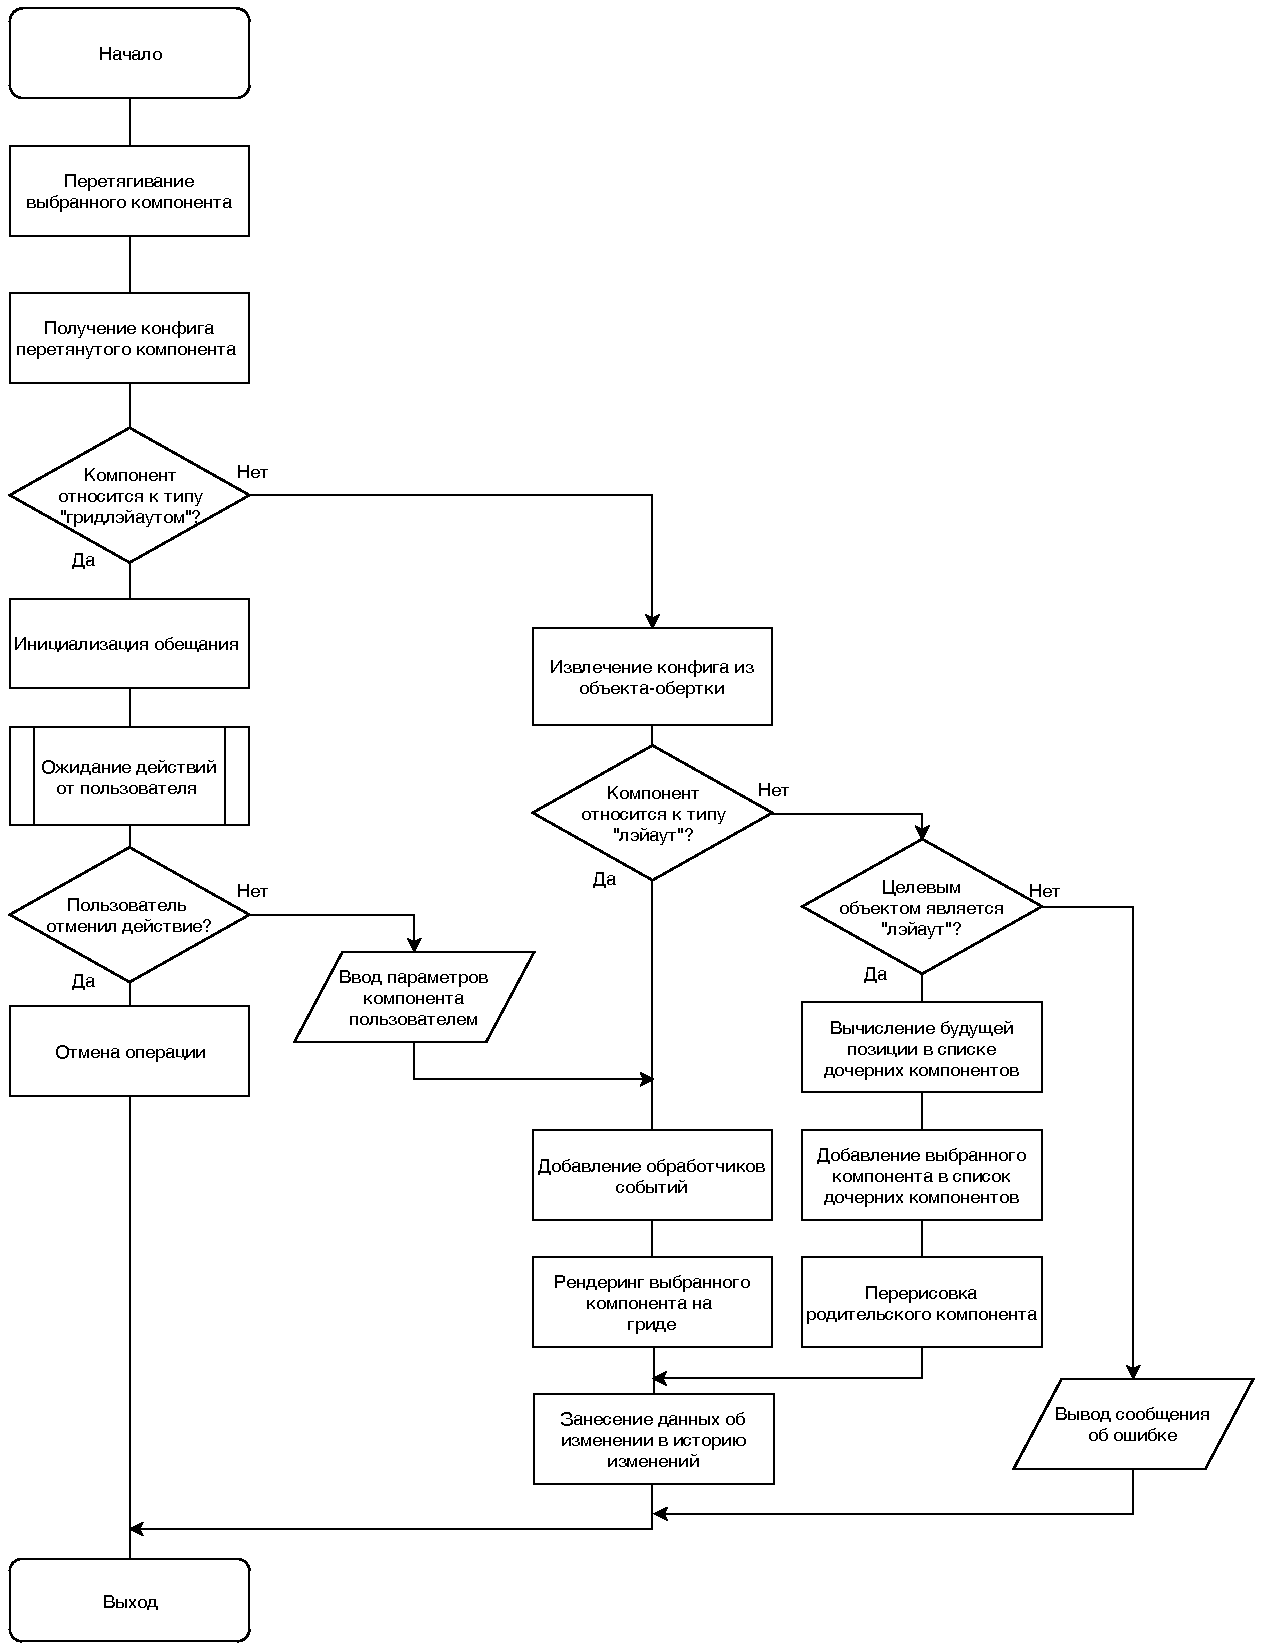
\includegraphics[scale=0.65]{composition.pdf}
    \caption{Алгоритм компоновки графических компонентов}
    \label{sec:dev:composition}
\end{figure}